\documentclass[a4paper]{article}

\usepackage[english]{babel}
\usepackage[utf8x]{inputenc}
\usepackage{amsmath}
\usepackage{amsfonts}
\usepackage{graphicx}
\usepackage[colorinlistoftodos]{todonotes}

\title{CS 5785 -- Applied Machine Learning -- Lec.\ 16}
\author{Prof.\ Nathan Kallus, Cornell Tech\\Scribe: TBD}
\date{Oct.\ 26, 2017 (Under construction)}

\begin{document}
\maketitle

\section{Decision Trees}

Decision trees partition the feature space into a set of rectangles.  We'll restrict our attention to trees with binary (two way) splitting nodes, which represent recursive binary partitions.  Decision trees can be used for regression or classification.  Fig.~\ref{fig:tree1} shows a regression example.  We can think of this as a tree-structured lookup table.  Bishop Fig.~\ref{fig:tree2} and \ref{fig:tree3} show examples for classification (categorical data).

\begin{figure}
\centering
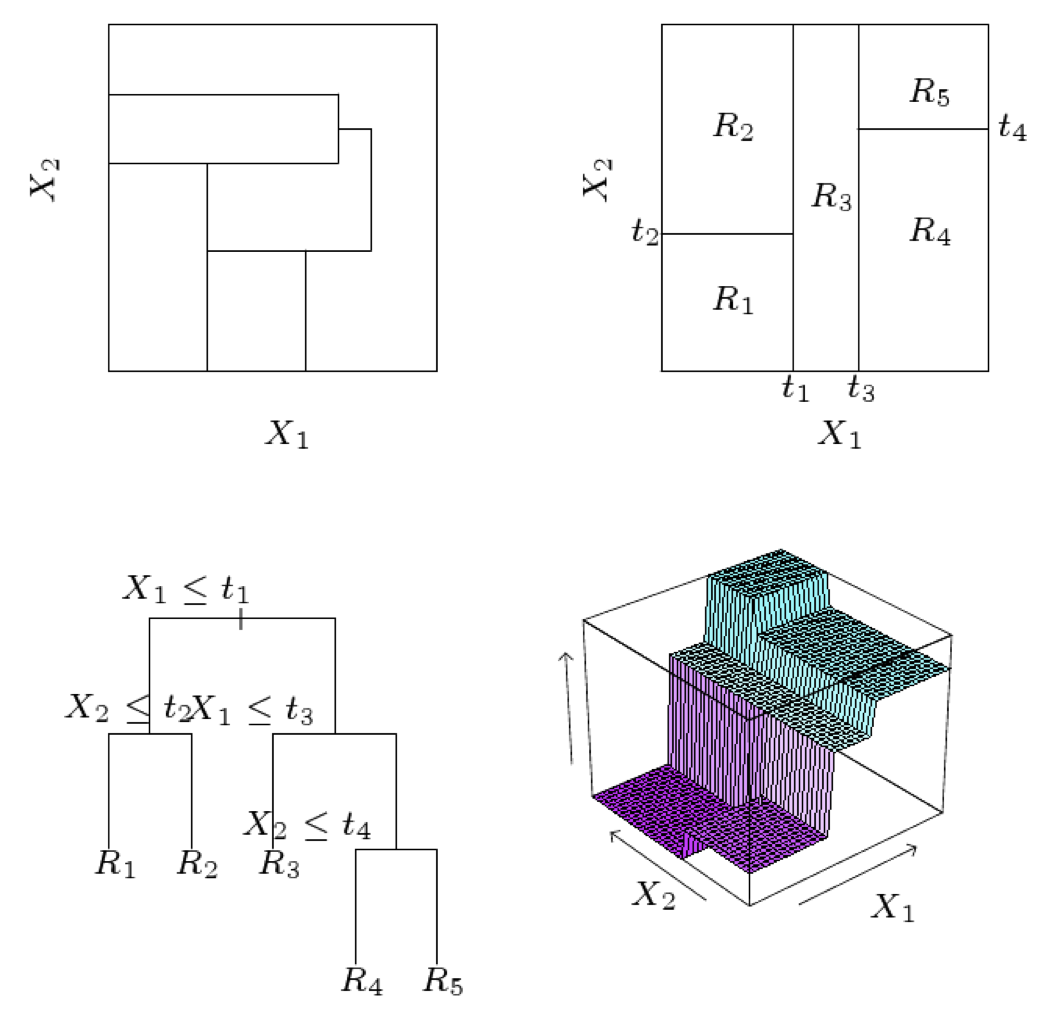
\includegraphics[width=1.0\textwidth]{fig9_2.png}
\caption{\label{fig:tree1}HTF Figure 9.2}
\end{figure}

\begin{figure}
\centering
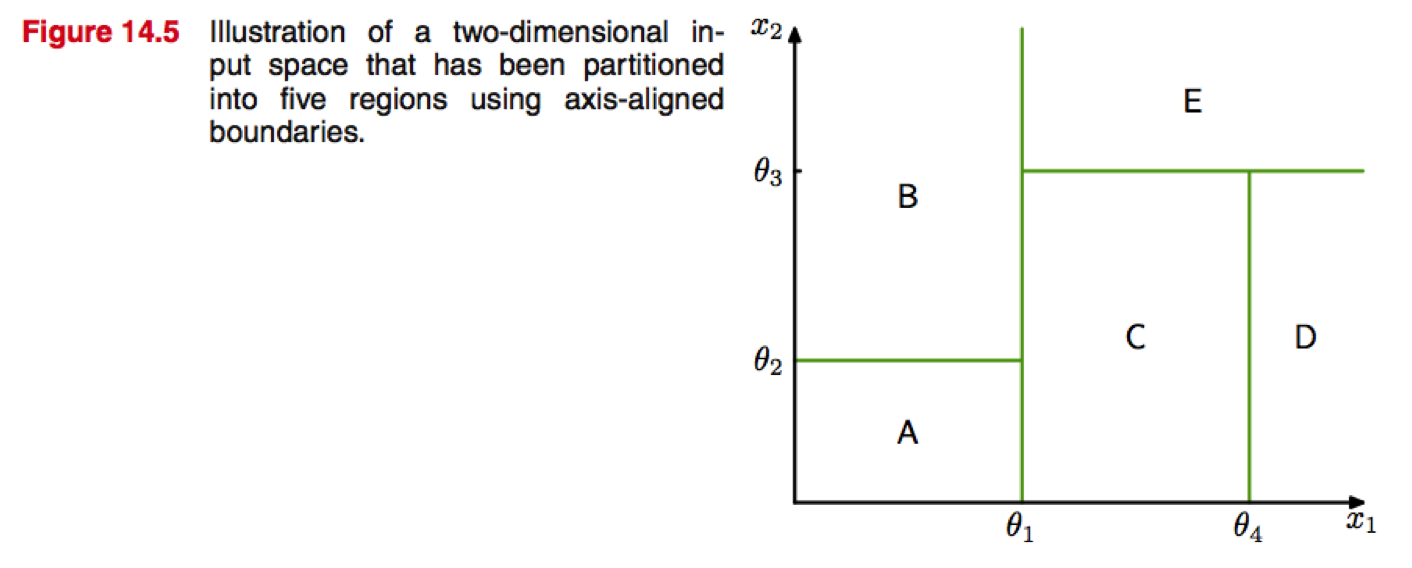
\includegraphics[width=1.0\textwidth]{fig14_5.png}
\caption{\label{fig:tree2}[Bishop]}
\end{figure}

\begin{figure}
\centering
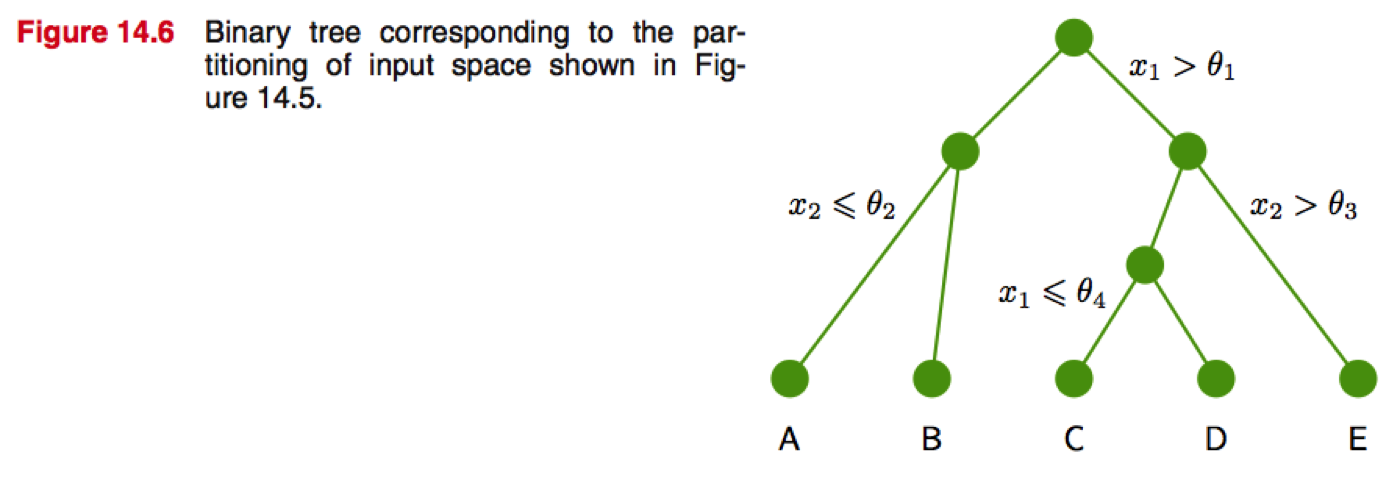
\includegraphics[width=1.0\textwidth]{fig14_6.png}
\caption{\label{fig:tree3}[Bishop]}
\end{figure}

We can write the regression model from Fig.~\ref{fig:tree1} as 
$$
\hat{f}(X) = \sum_{i=1}^5 c_m I\{(x_1,x_2) \in R_m\}
$$
where $I\{\cdot\}$ is an indicator function and $c_m$ gives us the constant value in each region.

We can express the equation above in tree form.  Terminal nodes (or leaves) correspond to the regions $R_m$.  The advantage of a tree is interpretability.  For example, it mimics how a doctor thinks.  It's much harder to draw partition diagrams for $p>2$ (partitions greater than 2) but that's not a problem for a tree.

We'll look first at regression trees, then classification trees.

\section{Regression Trees}

How do we grow a regression tree?  We're doing supervised learning so $Y$ is back in the picture.  There are $N$ observations, $( {x_i}, y_i)$, $i = 1, ..., N$, and $ {x_i} = (x_{i1}, x_{i2}, ..., x_{ip})$.

We need to decide how to split and what shape the tree should have.  Assume our model has the form
$$
f({x}) = \sum_{m=1}^{M} c_m I({x} \in R_m)
$$

How do we pick the $c_m$s?

If we use a sum of squares criterion, $\sum_i (y_i-f({x_i}))^2$, it's easy to show that the best $\hat{c}_m$ is obtained via averaging:
$$
\hat{c_m} = ave(y_i | {x_i} \in R_m)
$$
Finding the best binary partition according to this criterion, however, is in general computationally infeasible.  Let's try a greedy approach, which will get us the best splits in a decision tree. Remember that a decision tree only operates on one  variable at a time.

Pick a splitting variable $j$ and split point $s$, which induces a pair of half planes:
$$
R_1(j,s) = \{{X} | X_j \leq s\} \qquad \text{and} \qquad R_2(j,s) = \{{X}|X_j > s\}
$$
Then we want the $j$ and $s$ that solve
$$
\underset{j,s}{min} \left[\underset{c_1}{min} \sum_{{x_i} \in R_1(j,s)} (y_i-c_1)^2 + \underset{c_2}{min} \sum_{{x_i} \in R_2(j,s)} (y_i - c_2)^2\right]
$$
For a given choice of $j$ and $s$, the inner minimization is solved by:
$$
\hat{c}_1 = ave(y_i | {x_i} \in R_1(j,s)) \quad \text{and} \quad \hat{c}_2 = ave(y_i | {x_i} \in R_2(j,s))
$$
Scan over $j$, sweep through $s$ and pick the best split.  Repeat recursively. You are trying to approximate the elevation with two flat values around some splitting point.

How large a tree should we grow?  We want to hit a sweet spot: we don't want to miss important structure, but we also don't want to overfit (extreme case of one leaf node per data point).  Since it is a greedy method (i.e., it can get stuck at local optima), a lot of tree fitting algorithms involve some kind of randomization.

We can't be too short-sighted since there might be a seemingly worthless split that could lead to a very good split below it.  One popular strategy is to grow a tree to some fixed size and the prune it.  

We'll use something called \emph{cost-complexity pruning}.  Define a subtree $T \subset T_o$ to be any tree that can be obtained by pruning $T_o$, i.e., collapsing any number of its internal nodes.  The $m$th terminal node represents region $R_m$.  The number of terminal nodes in $T$ is denoted $\left\vert T\right\vert$.  \textit{N} represents the number of points inside a region.
$$
N_m = \# \{{x_i} \in R_m\}, \quad \hat{c}_m = \frac{1}{N_m} \sum_{{x_i} \in R_m} y_i, \quad Q_m(T) = \frac{1}{N_m} \sum_{{x_i} \in R_m} (y_i - \hat{c}_m)^2
$$
$Q_m(T)$ is an ``impurity measure'' and the cost-complexity criterion is given by
$$
C_\alpha(T) = \sum_{m=1}^{\left\vert T \right\vert} N_m Q_m(T) + \alpha \left\vert T \right\vert
$$
which is the weighted cost plus a ``complexity'' term.  Then we want to find, given an $\alpha \geq 0$, the subtree $T_\alpha \subseteq T_o$ to minimize $C_\alpha(T)$.  Tuning the parameter $\alpha$ controls the penalty on tree size:
big $\alpha$ gives us a small tree, small $\alpha$ yields up to a full tree ($\alpha = 0 \Rightarrow T_o$). 

We can choose $\alpha$ adaptively as follows.
For each $\alpha$, one can show that there is a unique smallest subtree $T_\alpha$ that minimizes $C_\alpha(T)$.
To find $T_\alpha$ use \emph{weakest link pruning}: successively collapse the internal node that produces the smallest per-node increase in the $\sum_m N_m Q_m(T)$ term above, and continue until we produce the single-node (root) tree.  The result is a finite sequence of subtrees.  One can show this sequence must contain $T_\alpha$ (details are omitted here).

Estimate $\alpha$ by 5- or 10-fold cross validation, i.e., choose $\hat{\alpha}$ to minimize the cross-validated sum of squares.  The final tree is $T_{\hat{\alpha}}$.  Now we've seen how to do regression using a binary tree.  How do we use trees for classification?

\section{Classification}

Now our target is a classification outcome, $1,2,...K$.  We just need to modify our criteria for splitting and pruning.  The squared error wouldn't make sense here.

Suppose we're at a node $m$ representing region $R_m$ with $N_m$ observations.  Let
$$
\hat{p}_{mk} = \frac{1}{N_m} \sum_{{x_i} \in R_m} I(y_i = k)
$$
In other words, $\hat{p}_{mk}$ represents the proportion of class $k$ observations in node $m$.

If you want to use the decision tree to make a choice, classify the observations in node $m$ to the majority class in node $m$:
$$
k(m) = \arg \max_k \hat{p}_{mk}
$$

Here are some choices for $Q_m(T)$ for ``node impurity'' that make sense for classification trees.
\begin{enumerate}
\item Misclassification error: $\frac{1}{N_m} \sum_{i \in R_m} I(y_i \neq k(m)) = 1-\hat{p}_{mk}(m)$
\item Gini index: $\sum_{k \neq k^\prime} \hat{p}_{mk} \hat{p}_{mk^\prime} = \sum_{k=1}^{K} \hat{p}_{mk}(1-\hat{p}_{mk})$
\item Cross-entropy/deviance: $-\sum_{k=1}^{K} \hat{p}_{mk} \log \hat{p}_{mk}$
\end{enumerate}

It's instructive to see what these reduce to in a 2-class case. The purest outcome you can have is that one of the labels has all of the observations piled into that class. Least pure (noisiest) option is where observations that fell into it could be any of the classes.  If $p$ is the proportion in class $2$, we have (at some node $m$) the following three node impurities:
$$
1-\max(p,1-p),\quad 2p(1-p),\quad -p\log p - (1-p) \log (1-p)
$$

\begin{figure}
\centering
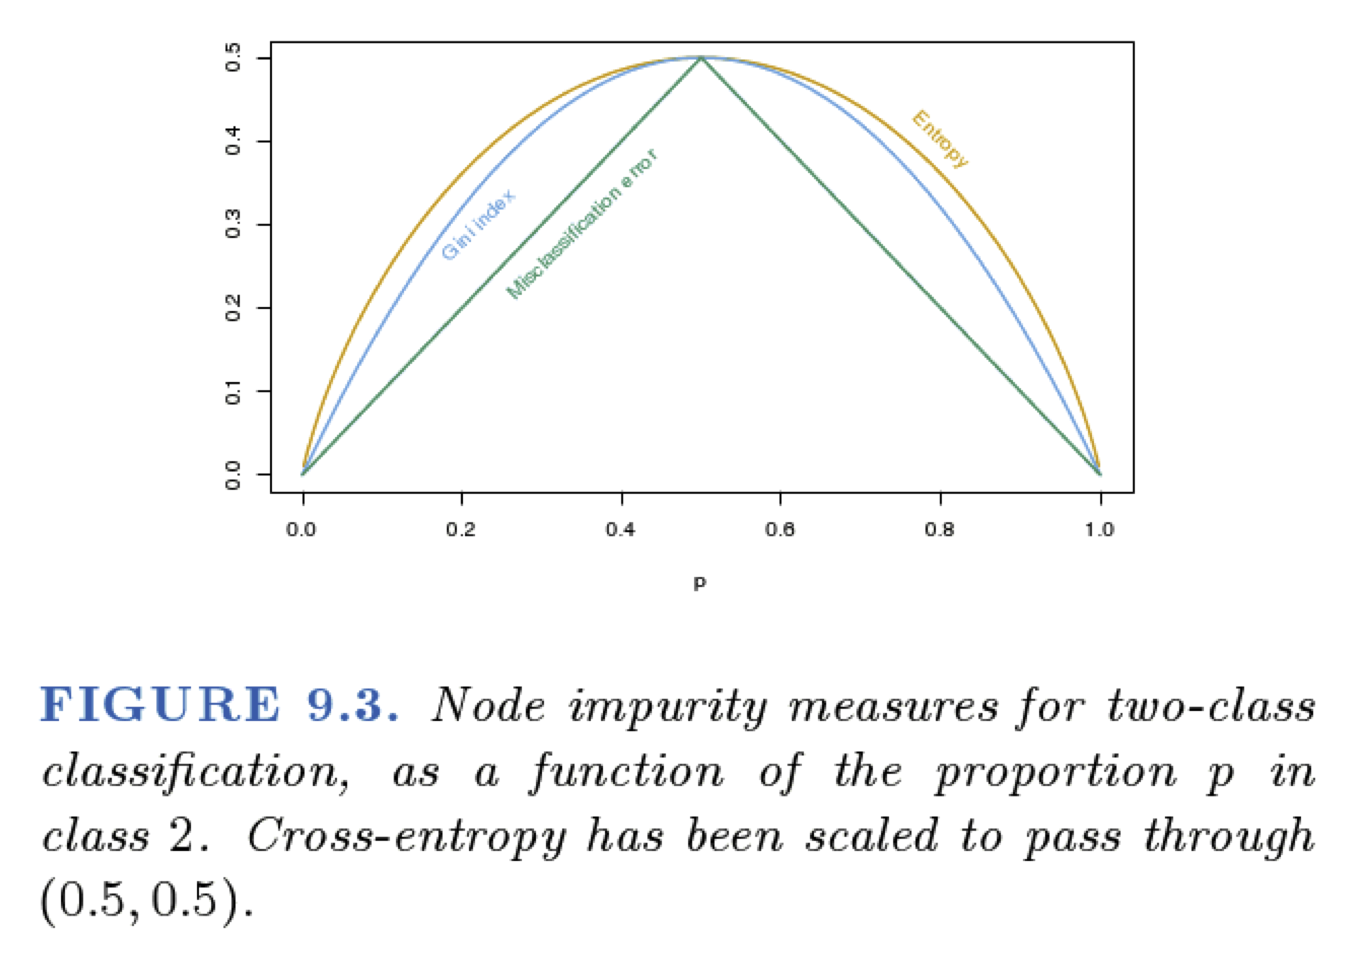
\includegraphics[width=1.0\textwidth]{fig9_3.png}
\caption{\label{fig:tree4} HTF Fig 9.3}
\end{figure}
These are illustrated in Fig.~\ref{fig:tree4}.  Note that Gini and cross-entropy are differentiable, which makes them well suited for numerical optimization.  
Minimizing cross entropy is equivalent to maximizing information gain between the test $X_j \leq s$ and the class label $Y$.
Gini and cross-entropy prefer ``pure'' nodes, i.e., nodes containing only one class.  Recall that entropy is a measure of uncertainty of a random variable, which makes it an intuitive choice for quantifying node impurity.

To see the contrast between these measures with simple misclassification error, suppose we have a 2-class problem with $400$ observations per class, denoted $(400, 400)$.
\begin{itemize}
\item One split creates nodes $(300,100)$ and $(100,300)$
\item Another creates nodes $(200,400)$ and $(200,0)$
\end{itemize}
The misclassification rate is the same for both splits: $0.25$.
If you compute the Gini index and cross-entropy, however, you'll see they prefer the second split since one of the resulting nodes is pure.  Gini or cross-entropy are usually used when growing a tree, but for cost-complexity pruning, the misclassification rate is usually used.


\begin{figure}
\centering
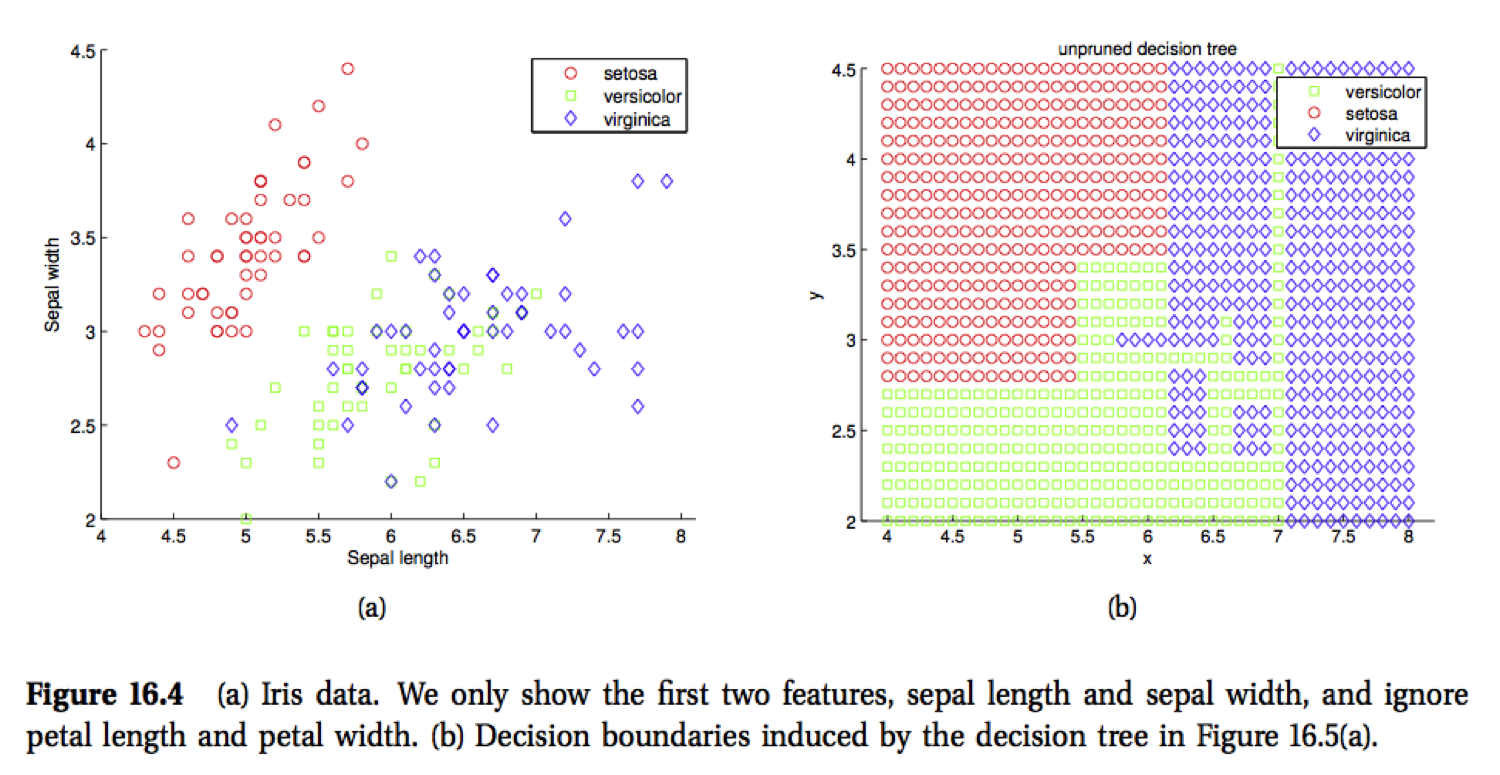
\includegraphics[width=1.0\textwidth]{fig16_4.png}
\caption{\label{fig:tree5}[Murphy]}
\end{figure}

\begin{figure}
\centering
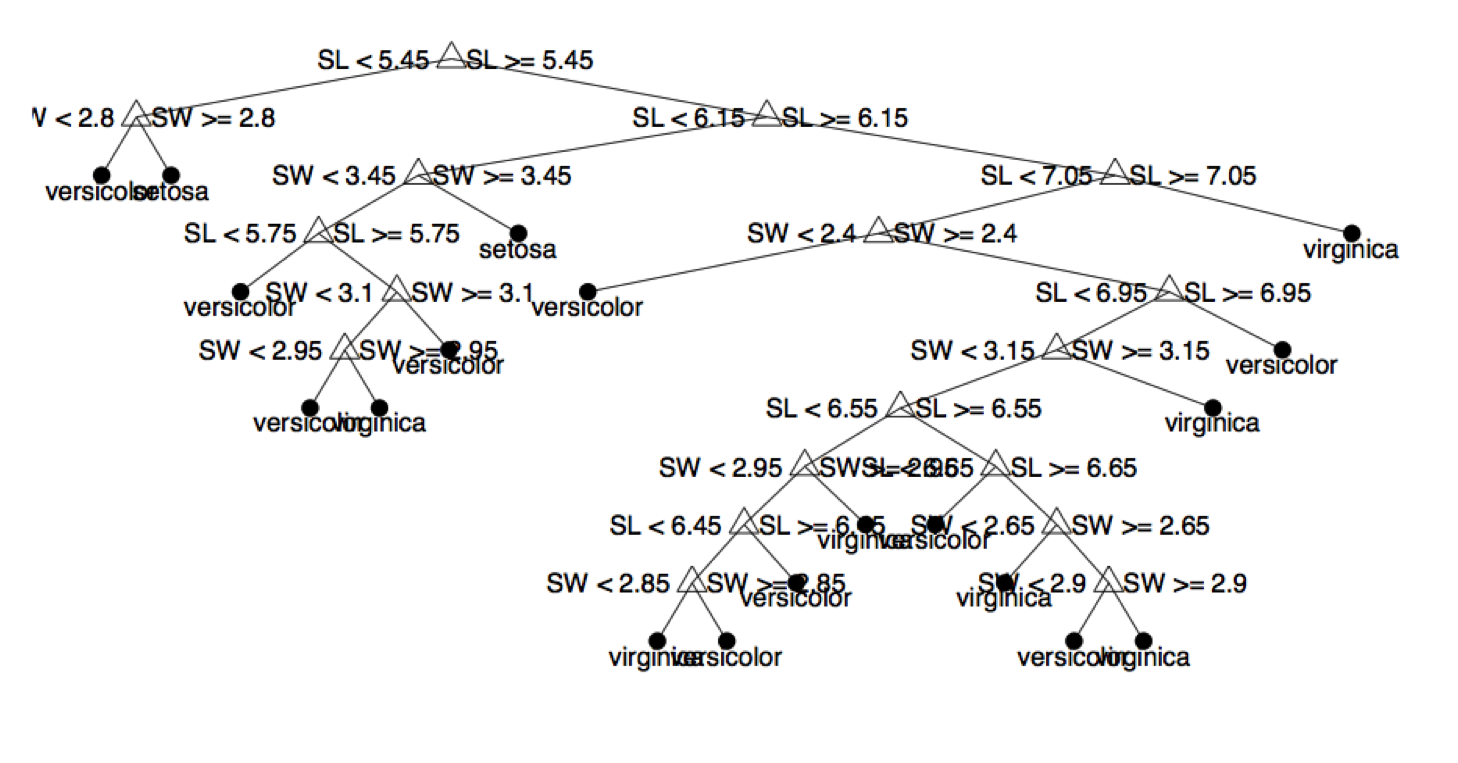
\includegraphics[width=1.0\textwidth]{fig16_5a.png}
\caption{\label{fig:tree6}[Murphy]}
\end{figure}

\begin{figure}
\centering
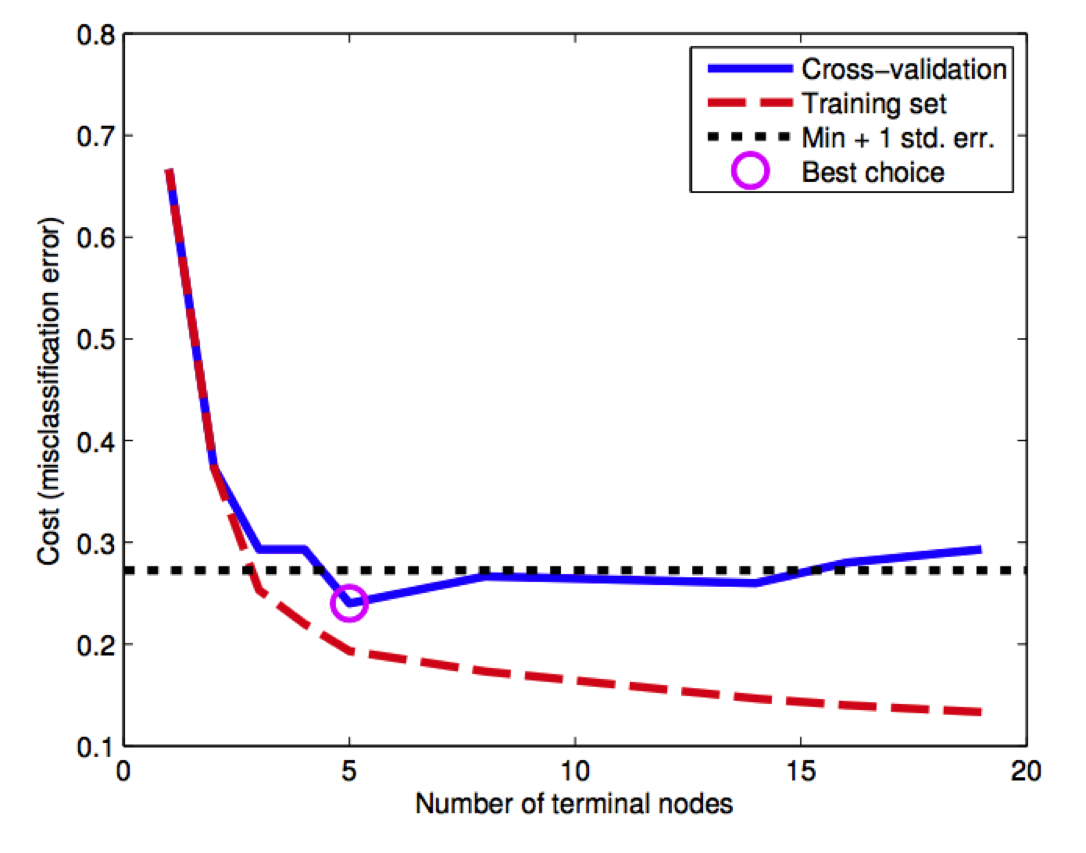
\includegraphics[width=1.0\textwidth]{fig16_5b.png}
\caption{\label{fig:tree7}[Murphy]}
\end{figure}

\begin{figure}
\centering
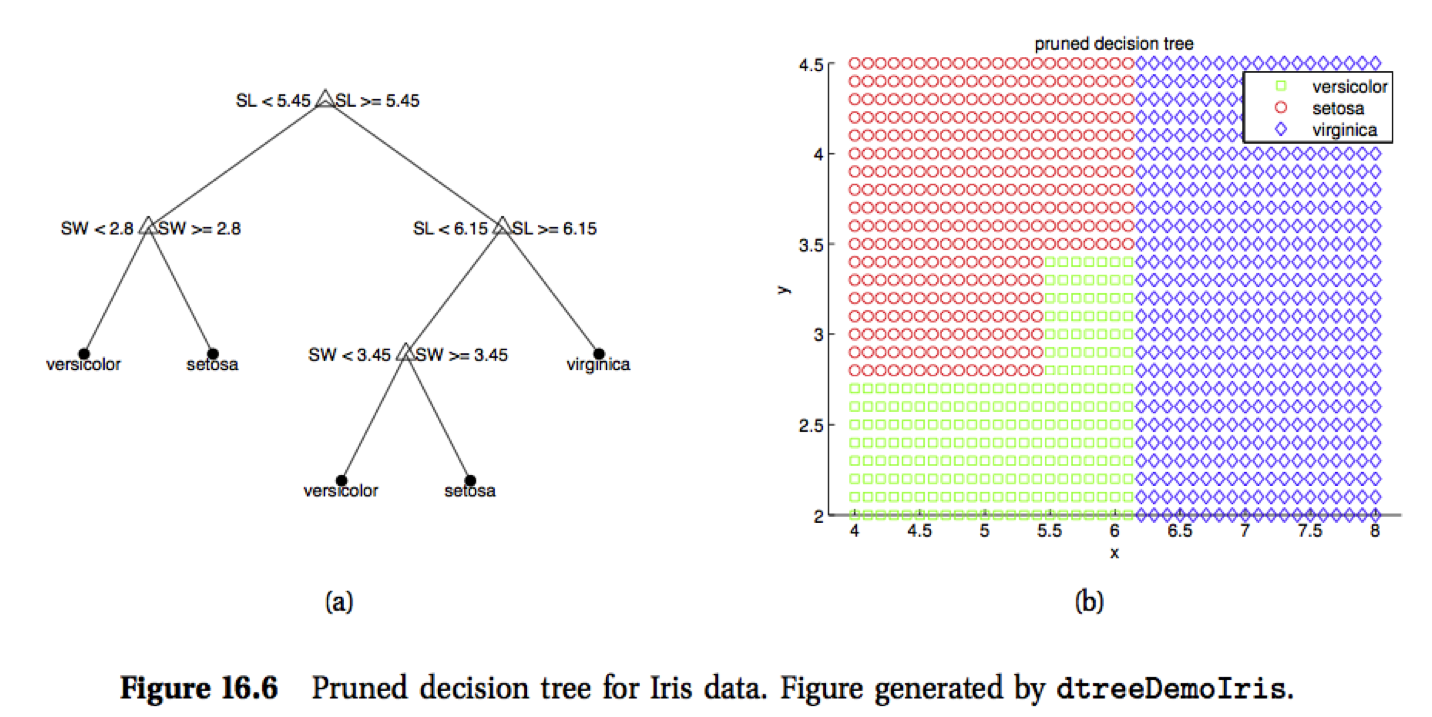
\includegraphics[width=1.0\textwidth]{fig16_6.png}
\caption{\label{fig:tree8}[Murphy]}
\end{figure}

Fig.~\ref{fig:tree5} illustrates the iris (flower) data set, a 3-class example.  We can use 2 of the 4 features -- sepal length and width -- to build an unpruned tree.  With $|T|=19$, the tree, shown in Fig.~\ref{fig:tree6}, looks very complex, with evidence of overfitting in the plot of error vs.~the number of terminal nodes $|T|$, shown in Fig.~\ref{fig:tree7}.
The pruned tree, shown in Fig.~\ref{fig:tree8}, has $\left\vert T \right\vert = 5$, and we can see by comparing it to the tree in Fig.\ref{fig:tree6} what pruning occurred.

This approach is called CART, for ``Classification and Regression Tree,'' and it is closely related to the software packages C4.5 and C5.0.

ADDITIONAL MATERIAL: For additional graphical visualization of decision trees, follow this link: http://www.r2d3.us/visual-intro-to-machine-learning-part-1/.

\end{document}
